\documentclass[10pt]{article}

% amsmath package, useful for mathematical formulas
\usepackage{graphicx,amsmath}
% amssymb package, useful for mathematical symbols
\usepackage{amssymb}

% cite package, to clean up citations in the main text. Do not remove.
\usepackage{cite}

\usepackage{hyperref}

% line numbers
\usepackage{lineno}

% ligatures disabled
\usepackage{microtype}
\DisableLigatures[f]{encoding = *, family = * }

% rotating package for sideways tables
% \usepackage{rotating}

% If you wish to include algorithms, please use one of the packages below.
% Also, please see the algorithm section of our LaTeX guidelines
% (http://www.plosone.org/static/latexGuidelines) for important information about
% required formatting.
% \usepackage{algorithmic}
% \usepackage{algorithmicx}

% Use doublespacing - comment out for single spacing
% \usepackage{setspace}
% \doublespacing

% Text layout
\topmargin 0.0cm
\oddsidemargin 0.5cm
\evensidemargin 0.5cm
\textwidth 16cm
\textheight 21cm

% Bold the 'Figure #' in the caption and separate it with a period % Captions
% will be left justified
\usepackage[labelfont=bf,labelsep=period,justification=raggedright]{caption}

% Use the PLoS provided BiBTeX style
\bibliographystyle{plos2015}

% Remove brackets from numbering in List of References
\makeatletter
\renewcommand{\@biblabel}[1]{\quad#1.}
\makeatother

% Leave date blank
\date{}

\pagestyle{myheadings}

%% Include all macros below. Please limit the use of macros.

%% END MACROS SECTION

\begin{document}

% Title must be 150 characters or less
\begin{flushleft}
	{\Large \textbf{????} } \\

	%Insert Author names, affiliations and corresponding author email.
 	Mason Liang$^{1,\ast}$,
	Rasmus Nielsen$^{2}$\\

	\bf{1} Mason Liang Integrative Biology, University of California, Berkeley, California, United States of America\\
	\bf{1} Rasmus Nielsen Integrative Biology, University of California, Berkeley, California, United States of America\\
	$\ast$ E-mail: wmliang@berkeley.edu
\end{flushleft}

% Please keep the abstract between 250 and 300 words
\section*{Abstract}
Estimating admixture histories is crucial for understanding the genetic
diversity we see in present-day populations. Existing allele frequency or
phylogeny-based methods are excellent for inferring the existence of admixture
or its proportions, but have less power for estimating admixture times. Recently
introduced approaches for estimating these times use spatial information from
admixed chromosomes, such as the local ancestry or the decay of admixture
linkage disequilibrium (ALD).  One popular method, implemented in the programs
ALDER and ROLLOFF, uses two-locus ALD to infer the time of a single admixture
event, but is only able to estimate the time of the most recent admixture event
based on this summary statistic.  We derive analytical expressions for the
expected ALD in a three-locus system and provide a new statistical method based
on these results that is able to resolve more complicated admixture histories.
Using simulations, we show how this new statistic behaves on a range of
admixture histories. As an example, we also apply our method to the Colombian
and Mexican samples from the 1000 Genomes project.

\section*{Introduction}
There are many methods for inferring the presence of
admixture, e.g. methods using simple summary statistics detecting deviations
from phylogenetic symmetry \cite{reich2009reconstructing} [TODO(mason) Also cite
patterson paper and paper from Monty's group], methods estimating admixture
proportions with programs such as Structure \cite{pritchard2000inference},
Admixture \cite{alexander2009fast} or RFmix \cite{maples2013rfmix}. However,
there has been less research on estimating admixture times,
possibly because such methods require data which were unavailable until the
advent of high-throughput next generation sequencing. Some recently developed
methods use the inferred local ancestry of sequences to construct admixture
tract length distributions, such as \cite{pool2009inference},
\cite{gravel2012population}, and \cite{liang2014lengths}.
Over time, recombination is expected to decrease the average lengths of admixture
tracts. The length distribution of admixture tracts is therefore informative
about the time since admixture.  Much of the theory relating to tracts lengths
is based on Fisher's famous theory of junctions \cite{fisher1949theory} and
subsequent work, such as
\cite{
	stam1980distribution,
	guo1994computation,
	bickeboller1996distribution,
	bickeboller1996probability,
	stefanov2000distribution,
	ball2005evaluation,
	cannings2003identity,
	dimitropoulou2003recsim,
	walters2005probability,
	rodolphe2008theoretical
}.
For example, \cite{baird2003distribution} first
discussed the length distribution of tracts descended from a single ancestor.
These results informed later analyses of admixture tract length distribution,
such as \cite{pool2009inference}, \cite{gravel2012population}, and
\cite{liang2014lengths}. \cite{gravel2012population} also implemented the
software program TRACTS, which estimates admixture histories by fitting the
tract length distribution, obtained by local ancestry inference, to a
exponential approximation.

Another approach, which we will follow in this paper, is based on the decay of
admixture linkage disequilibrium (ALD). In a well-mixed, genetically isolated
human populations, linkage disequilibrium decays to zero on a scale of tenths of
centiMorgans. However, when an admixed population is founded, it begins with
large of amount of linkage disequilibrium, which is a result of the allele
frequency differences between the source populations. This occurs even if the LD
in the source populations themselves is negligible. The linkage disequilibrium
in the admixed population then fluctuates in the generations after its founding,
decreasing as a result of drift and recombination, or increasing because of
additional waves of migration. From the LD present in a modern day admixed
population, it is possible to make inferences about the population's admixture
history. This insight was first used in the program ROLLOFF
\cite{moorjani2011history} and was later extended by ALDER
\cite{loh2013inferring}.

These two methods use the fact that if an admixed population takes in no
additional migrants after the founding generation, the LD present in the
population is expected to decay exponentially as a function of distance. The
rate constant of this exponential decay is proportional to the age of the
founding admixture pulse and so can be used as an estimator. ROLLOFF and ALDER
are well suited for inferring the time of the admixture event when the
population's admixture history can be approximated as a single pulse. However,
it can be important to estimate parameters for admixture histories involving
multiple pulses, such as estimating the date of Native American admixture in
Rapa Nui \cite{moreno2014genome} or determining migration patterns in the
Americas \cite{gravel2013reconstructing}. In these instances the expected decay
of LD will become a mixture of exponentials. ROLLOFF and ALDER have limited
resolution, as they can usually only infer the date of the most recent migration
wave \cite{moorjani2011history}, or reject the hypothesis of a single pulse
admixture \cite{loh2013inferring}.

ROLLOFF and ALDER use the information contained in pairs of sites by examining
the two-locus linkage disequilibrium between them. Here we extend the theory
underlying the methods in ROLLOFF and ADLER to three loci by considering
three-locus LD. There are two ways of measuring the linkage between $n$ loci.
\cite{bennett1952theory} defines $n$-locus linkage in a way that maintains a
geometric decrease of LD each generation as a result of recombination, which is
an important property of two-locus linkage disequilibrium.
\cite{slatkin1972treating} defines $n$-locus LD  to be the $n$-way covariance,
analogously to the property of two locus LD as the covariance in allele
frequency between pairs of loci. For two and three loci, these two definitions
coincide, but for four or more loci, they do not.

In this paper, we will use Bennett and Slatkin's definition of three-locus LD to
examine the the decay of ALD for three sites as a function of the genetic
distance between them. We derive an equation that describes the decay of
three-locus LD under an admixture history with multiple waves of migration. We
then compare the results of coalescent simulations to this equation, and develop
some guidelines for when admixture histories more complex than a single pulse
can be resolved. Finally, we apply our method to the Colombian and Mexican
samples in the 1000 Genomes data set, using the Yoruba samples as a reference.
Fitting a two-pulse model to data, we estimate admixture histories for the two
populations which are qualitatively consistent with the results reported in
\cite{gravel2013reconstructing}.

[TODO Could we say anything here about Neanderthals in Asia?]

% You may title this section "Methods" or "Models". % "Models" is not a valid
title for PLoS ONE authors. However, PLoS ONE % authors may use "Analysis"
\section{Model} We use a random union of gametes admixture model as described in
\cite{liang2014understanding}, which is an extension of the mechanistic
admixture model formulated by \cite{verdu2011general}. In this model, two or
more source populations contribute migrants to form an admixed population
consisting of $2N$ haploid individuals. Each generation in the admixed
population is formed through the recombination of randomly selected individuals
from the previous generation, with some individuals potentially replaced by
migrants from the source populations. For simplicity, we consider a model with
only two source populations. Furthermore, the first source population only
contributes migrants in the founding generation, $T$. The second source
population contributes migrants in the founding generation and possibly in one
or more generations thereafter. In generation $i$, for $i=T-1,\dots,0$ (before
the present), a fraction $m_i$ of the admixed population is replaced by
individuals from the second source population.

\section{Linkage Disequilibrium and Local Ancestry} ROLLOFF and ALDER use the
standard two-locus measure of LD between a SNP at positions $x$ and another SNP
at position $y$, which is a genetic distance $d$ to the right,

\begin{align} D_2(d) = \text{cov}(H_x,H_y), \label{D2} \end{align}

where $H_x$ and $H_y$ represent the haplotype or genotypes of an admixed
chromosome at positions $x$ and $y$. In the case of haplotype data, $H_{i,x}=1$
if the $i^\text{th}$ sample is carrying the derived allele at the SNP at
position $x$, and is otherwise 0. Alternatively, for genotype data, $H_{i,x}$
take on values from $\{0,1/2,1\}$ depending on the number of copies of the
derived allele the $i^\text{th}$ sample is carrying at SNP position $x$. We
consider an additional site at position $z$, which is located a further genetic
distance $d'$ to the right of $y$. The three-loci LD, as defined by as defined
by \cite{bennett1952theory} and \cite{slatkin1972treating}, is given by

\begin{align} D_3(d,d') = \text{cov}(H_x,H_y,H_z) =
\mathbb{E}[(H_x-\mathbb{E}H_x)(H_y-\mathbb{E}H_y)(H_z-\mathbb{E}H_z)].
\label{D3} \end{align}

The LD in an admixed population depends on the genetic differentiation between
the source populations and and its admixture history. Let $A_x$ represent the
local ancestry at position $x$, with $A_x=1$ if $x$ is inherited from an
ancestor in the first source population, and $A_x=0$ if $x$ is inherited from
the second source population. We can compute $D_3$ in terms of the three-point
covariance function of $A_x$ and so separate out the effects of allele
frequencies and local ancestry. Let $H_x = f_x+\delta A_x$, where $f_x$ is the
allele frequency of locus $x$ in the first source population and $\delta_x$ is
the difference of the allele frequencies of locus $x$ in the two source
populations. We now make the assumption that the allele frequencies in the
source populations are known and fixed. Equation \ref{D3} then becomes

\begin{align} D_3(d,d') &=
\text{cov}\left(f_x+\delta_xA_x,f_y+\delta_yA_y,f_z+\delta_zA_z\right)\nonumber \\ &=
\delta_x\delta_y\delta_z \text{cov}(A_x,A_y,A_z). \label{local_ancestry}
\end{align} A similar argument shows that $D_2(d)$ is proportional to the
two-point covariance function of the local ancestry.

\subsection{Local Ancestry Covariance Functions} From the above section we see
that we can describe the three-point admixture LD in terms of covariances of
local ancestry in the three points.  We now expand the covariance in equation
\ref{D3} into its component expectations to get \begin{align*}
\text{cov}(A_x,A_y,A_z) &= \mathbb{E}[A_xA_yA_z]
-\mathbb{E}[A_xA_y]\mathbb{E}[A_z] -\mathbb{E}[A_xA_z]\mathbb{E}[A_y]
-\mathbb{E}[A_yA_z]\mathbb{E}[A_x]
+2\mathbb{E}[A_x]\mathbb{E}[A_y]\mathbb{E}[A_z]. \end{align*} Each one of these
expectations on the right-hand side is the probability that one or more sites is
inherited from an ancestor from first source population. We organize these
products of probabilities in a column vector: \begin{align*} \mathbf{v}_3 &=
\left(\begin{array}{l} \mathbb{P}\{A_x=A_y=A_z=1\}\\
\mathbb{P}\{A_y=A_z=0\}\mathbb{P}\{A_x=0\}\\
\mathbb{P}\{A_x=A_z=0\}\mathbb{P}\{A_y=0\}\\
\mathbb{P}\{A_x=A_y=0\}\mathbb{P}\{A_z=0\}\\
\mathbb{P}\{A_x=0\}\mathbb{P}\{A_y=0\}\mathbb{P}\{A_z=0\} \end{array}\right),
\end{align*} so that $\text{cov}(A_x,A_y,A_z) = (1,-1,-1,-1,2)\mathbf{v}_3$.
There is one entry in $\mathbf{v}_3$ for each of the five ways in which the
three markers at positions $x,y$, and $z$ can arranged on one or more
chromosomes. In the founding generation $T$, this column vector is given by
$\mathbf{v}_{3(T)} = (1-m_T,(1-m_T)^2,(1-m_T)^2,(1-m_T)^2,(1-m_T)^3)'$. The
probabilities for subsequent generations can be found by left-multiplying drift,
recombination, and migration matrices: \begin{align*} \mathbf{v}_{3(i)} =
\mathbf{D}_i \mathbf{L}\mathbf{U} \mathbf{v}_{3(i-1)}, \end{align*} The matrices
$\mathbf{D}_i$, $\mathbf{L}$, and $\mathbf{U}$ account for the effects of
migration, drift, and recombination, respectively. The migration matrix is a
diagonal matrix given by \begin{align*} \mathbf{D}_i &=
\text{diag}(1-m_i,(1-m_i)^2,(1-m_i)^2,(1-m_i)^2,(1-m_i)^3). \end{align*} Its
entries are the probabilities that one, two, or three chromosomes in the admixed
population will not be replaced by chromosomes from the second source population
in generation $i$. The lower triangular drift matrix \begin{align*}
\mathbf{L}&=\frac{1}{4N^2}\left( \begin{array}{ccccc} 4N^2 		& 0 	& 0 & 0 & 0\\
2N 	& 2N(2N-1) & 0 & 0 & 0\\ 2N 	& 0 & 2N(2N-1) & 0 & 0\\ 2N 	& 0 & 0 & 2N(2N-1) &
0\\ 1 & 2N-1 & 2N-1 & 2N-1 & (2N-1)(2N-2) \end{array} \right) \end{align*} gives
the standard Wright-Fisher drift transition probabilities between the states as
a function of the population size $2N$. Finally, the upper triangular
recombination matrix is determined by the recombination rates between the three
sites: \begin{align*} \mathbf{U} &= \left( \begin{array}{ccccc} e^{-d-d'} &
(1-e^{-d})e^{-d'} & (1-e^{-d})(1-e^{-d'}) & e^{-d}(1-e^{-d'}) & 0 \\ 0 & e^{-d'} &
0 & 0 & 1-e^{-d'} \\ 0 & 0 & 1-e^{-d}-e^{-d'}+2e^{-d-d'} & 0 &
e^{-d}+e^{-d'}-2e^{-d-d'} \\ 0 & 0 & 0 & e^{-d} & 1-e^{-d} \\ 0 & 0 & 0 & 0 & 1
\end{array} \right) \end{align*} The covariance function is then given by
\begin{align} \text{cov}(A_x,A_y,A_z) &=
\left(1,-1,-1,-1,2\right)\left(\prod_{i=0}^{T-1} \textbf{D}_i
\mathbf{L}\mathbf{U}\right)\textbf{v}_{3(0)}. \label{cov} \end{align} We can
obtain an analogous equation for $\text{cov}(A_x,A_y)$, involving the migration,
drift, and recombination matrices for two loci: $$ \text{cov}(A_x,A_y) =
\left(1,-1\right)\left(\prod_{i=0}^{T-1} \textbf{D}_i
\mathbf{L}\mathbf{U}\right)\textbf{v}_{2(0)}. $$

In some cases, equation \ref{cov} simplifies further. In a one-pulse migration
model, in which $m_T=M$ and is there after 0, the $\mathbf{D}_i$'s become
identity matrices, and we get the closed from expression $$
\text{cov}(A_x,A_y,A_z) =
M(1-M)(1-2M)\left(1-\frac{1}{2N}\right)^T\left(1-\frac{2}{2N}\right)^Te^{-T(d+d')}. $$
This is because $(1,-1,-1,-1,2)$ is a left eigenvector of both $\mathbf{L}$ and
$\mathbf{U}$, with corresponding eigenvalues $(1-1/2N)(1-2/2N)$ and
$\exp(-d-d')$. Note that when $M=0$, the covariance function will be identically
0. Another case is a two pulse model in which we ignore the effects of genetic
drift. In this model, admixture only occurs $T$ and $T_2$ generations before the
present, so that $m_T=M_1,m_{T'}=M_2$, and all other $m_i$'s are 0. Making the
substitution $T_1=T-T_2$, the right hand side of equation \ref{cov} becomes
\begin{align}
&(1-M_1)(1-M_2)e^{-T_2(d+d')}\left[M_2(1-M_1)^2-2M_2^2(1-M_1)^2+M_1(1-2M_1)e^{-T_1(d+d')}\right.\nonumber\\ &\ \
\left.-M_1M_2(1-M_1)\left(e^{-M_1d}+e^{-M_1
d'}+\left(1-e^{-d}-e^{-d'}+2e^{-d-d'}\right)^{T_1}\right) \right]. \label
{ash_2p} \end{align} The corresponding expression for the two-point covariance
function is given by \begin{align}
(1-M_1)(1-M_2)e^{-T_2d}\left(M_2-M_1M_2+M_1e^{-T_1d}\right), \label{alder_2p}
\end{align} which is a mixture of two exponentials.

\section{Weighted Linkage Disequilibrium} As \cite{loh2013inferring} noted, we
cannot use the LD in the admixed population directly, because the allele
frequency differences in the source populations can be of either sign. As in
\cite{loh2013inferring} , we solve this problem by computing the product of the
values of the three-point linkage disequilibrium coefficient with the product of
the allele frequency differences. Using equation \ref{local_ancestry} we obtain $$
\delta_x\delta_y\delta_z
D_3(d,d')=\delta_x^2\delta_y^2\delta_z^2\mathbb{E}[\text{cov}(A_x,A_y,A_z)], $$
because the local ancestry in the admixed sample is independent of the allele
frequencies in the admixed population. For inference purposes, we estimate this
function by averaging over triples of SNPs which are separated by distances of
approximately $d$ and $d'$. The LD term is estimated from the admixed
population, while the $\delta$'s are estimated from reference populations which
are closely related to the two source populations. We notice that both this
approach, as well as the previous approaches (e.g., \cite{loh2013inferring} ),
does not take genetic drift in the source populations after the time of
admixture into account, i.e. there is an assumption of both this method and
previous methods that the allele frequencies in the ancestral source populations
can be approximated well using the allele frequencies in the extant populations.

We arrange the data from the admixed samples in an $n\times S_n $ matrix
$\mathbf{H}$, where $n$ is the number of admixed haplotypes/genotypes, and $S_n$
is the number of segregating sites in the sample. For ease of notation, we
assume that the positions are given in units which make the unit interval equal
to the desired bin resolution.

For a given $d$ and $d'$ the set of SNP triples we use in the estimator for the
weighted LD is $$ S[d,d'] = \left\{x,y,z: d\leq  x-y < d+1 \text{ and } d' \leq
y-z < d'+1 \right\}. $$ Let $f_x$ be empirical allele frequency in the admixed
population. An unbiased estimator of the weighted three-point linkage
disequilibrium coefficient is then \begin{align*} \hat{a}[d,d']&=
\frac{1}{|S[d,d']|} \sum_{x,y,z\in S[d,d']}\frac{n\sum_{i=1}^n
\delta_x\delta_y\delta_z(H_{i,x}-f_x)(H_{i,y}-f_y)(H_{i,z}-f_z)}{(n-1)(n-2)}.
\end{align*}

\section{Algorithm}
Directly computing $\hat{a}[d,d']$ over the set $d,d'\in \{0,1,\dots,P\}^2$
would be cubic in the number of segregating sites. However, by using the fast
Fourier Transform (FFT) technique introduced in ALDER \cite{loh2013inferring},
we can approximate $\hat{a}$ with an algorithm whose time complexity is instead
linear in the number of segregating sites.

First, rearrange $\hat{a}$ to get
\begin{align*}
	\hat{a}[d,d'] &=
	\frac{n}{(n-1)(n-2)}
	\frac{
		\sum_{i=1}^n \sum_{x,y,z\in S[d,d']}
		\delta_x \delta_y \delta_z (H_{i,x} - f_x) (H_{i,y} - f_y) (H_{i,z} - f_z)
	}{
		\sum_{x,y,z \in S[d,d']}
		1
	},
\end{align*}
and define sequences $b_i[d]$ and $c[d]$ by binning the data and then doubling
the length by padding with $P$ zeros,
\begin{align*}
	b_i[d] &=
	\left\{
		\begin{array}{ll}
			\sum_{x: d\leq \lfloor{x}\rfloor < d+1} \delta_x(H_{i,x}-f_x) & : 0 \leq d < P\\
			0 & : P\leq d <2P
		\end{array}
	\right.\\
	c[d] &=
	\left\{
		\begin{array}{ll}
			|\{x: d\leq \lfloor{x}\rfloor < d+1\}| & : 0\leq d < P\\
			0 & : P\leq d <2P
		\end{array}
	\right.
\end{align*}
We can approximate $|S[d,d']|$ and the $n$ sums in the numerator of
$\hat{a}[d,d']$ in terms of convolutions of these sequences:
$$
	|S[d,d']| \approx \sum_{w=0}^P c[w]c[w+d]c[w+d+d']
$$
$$
	\sum_{x,y,z\in S[d,d']}
	\delta_x\delta_y\delta_z(H_{i,x}-f_x)(H_{i,y}-f_y)(H_{i,z}-f_z)
	\approx
	\sum_{w=0}^P b_i[w]b_i[w+d]b_i[w+d+d'].
$$
These convolutions can be efficiently
computed with an FFT, since under a two-dimensional discrete Fourier transform
from $(d, d')$-space to $(j, k)$-space,
$$
\sum_{w=0}^P b_i[w]b_i[w+d]b_i[w+d+d']
\leftrightarrow
B_i[j]\bar{B_i}[k]B_i[k-j],
$$
where $B_i$ is the one-dimensional discrete Fourier transform of $b$ and for
$j>0$, $B_i[-j]$ is the $j^\text{th}$ to last most element of $B_i$.
Summing over $i$ and taking the inverse discrete Fourier transform, we can
approximate the discrete Fourier transform of the numerator of $\hat{a}$. We
apply the same method to $c$ to approximate the denominator of $\hat{a}$.

The time complexities for the binning and the FFT's are $O(S_n)$ and
$O(P^2\log(P))$. Of these two, the first term will dominate, because $P$, the
number of bins, much less than $S_n$, the number of segregating sites.

When only one source population is available,

When using only the admixed population itself as a reference population, the
method described above will be biased if the same samples are used to estimate
both the linkage disequilibrium coefficients and the weights ($\delta_x$,
$\delta_y$, and $\delta_z$). We cannot efficiently compute a polyache statistics
like \cite{loh2013inferring}. At the cost of some power, we instead adopt the
approach of \cite{pickrell2012inference} and separate the admixed population
into two equal-sized groups. We then use one group to estimate the weights, and
the other group to estimate linkage disequilibrium coefficients, and vice versa.
This gives gives two unbiased estimates for the numerator of $\hat{a}$, which we
then average. [TODO Comment: I didn't understand how this works.  Coudl we five
more detail?] \subsection{Fitting the Two-Pulse Model} We fit equation
\ref{alder_2p} to the estimates of the weighted LD using non-linear least
squares, with two modifications. We added a proportionality constant to account
for the expected square allele frequency difference between the source
populations. We also subtracted out an affine term in the weighted LD which is
due to population substructure \cite{loh2013inferring}. We estimated this by
computing the three-way covariance between triples of chromosomes. We use the
jackknife to obtain confidence intervals for the resulting estimates by leaving
out each chromosome in turn and refitting on the data for the remaining
chromosomes.  [TODO Comment: again, we need more detail here. These are
important parts of the manuscript] \section{Simulations} We used the program
macs \cite{chen2009fast} to generate two source populations which diverged 4000
generations ago and a coalescent simulation to generate an admixed population
from the two source populations according to two-pulse and constant admixture
models. We sampled 50 diploid individuals from the admixed and two source
populations, each consisting of 20 chromosomes of length 1 Morgan. The effective
population size was $2N=1000$ for the admixed population and two source
populations. Using a two pulse model, we varied the migration probabilities and
timings for each pulse to examine the accuracy of equation \ref{alder_2p}. We
also simulated data for a model with a constant rate of admixture each
generation, and compared this to the predictions made by equation \ref{cov}.
\section{Data Set} We computed the weighted LD for the Mexican and Columbia
populations in the first phase of the 1000 Genomes data set. These consisted of
66 individuals from Los Angeles and 60 individuals from Medellin, respectively.
We used the 88 Yoruba samples as the one reference population. We computed the
weighted LD on the genotypes to avoid effects of phasing errors. % Results and
Discussion can be combined. \section{Results and Discussion} % We only support
three levels of headings, please do not create a heading level below
\subsubsection. \subsection{Simulations}

\begin{figure} 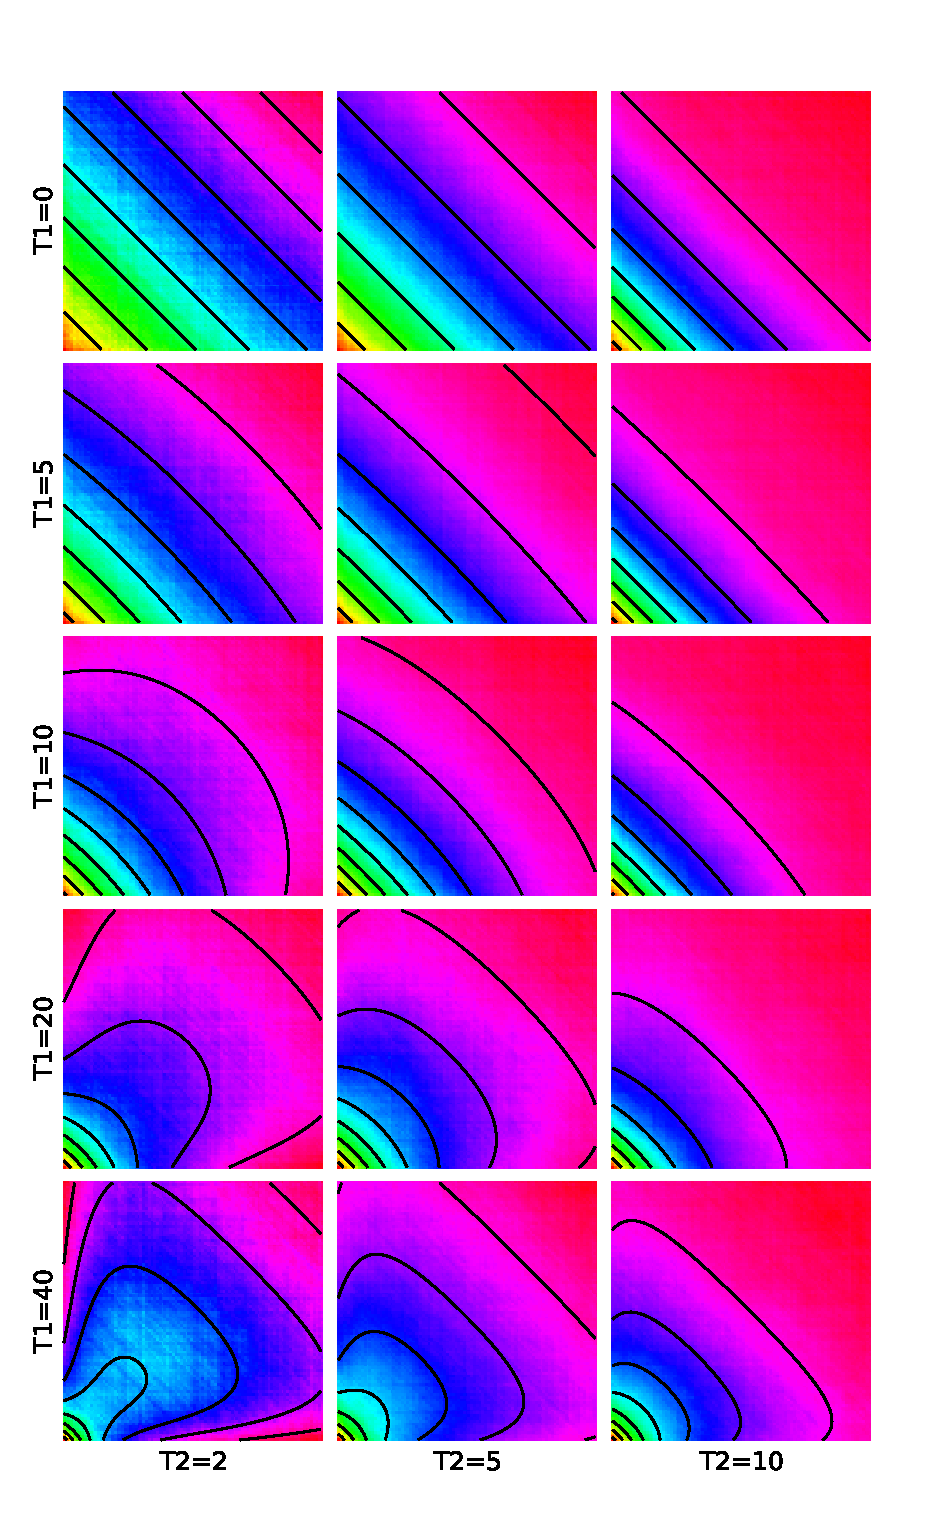
\includegraphics[scale=.6]{Ts.eps}\caption{ {\bf Predicted
weighted LD surfaces from simulations and theory for varying admixture times.}
The heat maps are from simulations and the contours are plotted from equation
\ref{D3}. The two admixture probabilities were fixed at $m_1=m_2=.2$ and the the
times of the two admixture pulses, $T_1$ and $T_2$, were varied. Each square
covers the range $0.5 \text{ cM }<d,d'<20\text{ cM}$. When time of the more
recent pulse is greater than half of that of the more ancient pulse, i.e.
$2T_1>T_1+T_2$, the contours of the resulting weighted LD surface are straight,
making it difficult to distinguish from the weighted LD surface produced by a
one-pulse admixture scenario. } \label{Ts} \end{figure}

[TODO: the color coding should be labeled for all figures.  Also, the y and
x-axes should be labeled]

\begin{figure} \includegraphics[scale=.6]{ms.eps} \caption{ {\bf Predicted
weighted LD surfaces from simulations and theory for varying admixture
proportions.} The heat maps are from simulations and the contours are plotted
from equation \ref{D3}. The two admixture times were fixed at 2 and 12
generations ago ($T_1=10$ and $T_2=2$) while the admixture probabilities were
varied. Each square covers the range $0.5 \text{ cM }<d,d'<20\text{ cM}$. As the
total admixture proportion $m_2+m_1(1-m_2)$ increases above 0.5, the contours
change to reflecting that the majority contribution of the genetic material now
originates from the other population. Weighted LD surfaces for $m_1>0.5$ or
$m_2>0.5$ are not shown, but are qualitatively similar to the surfaces on the
lower and rightmost sides. } \label{ms} \end{figure}

\begin{figure} 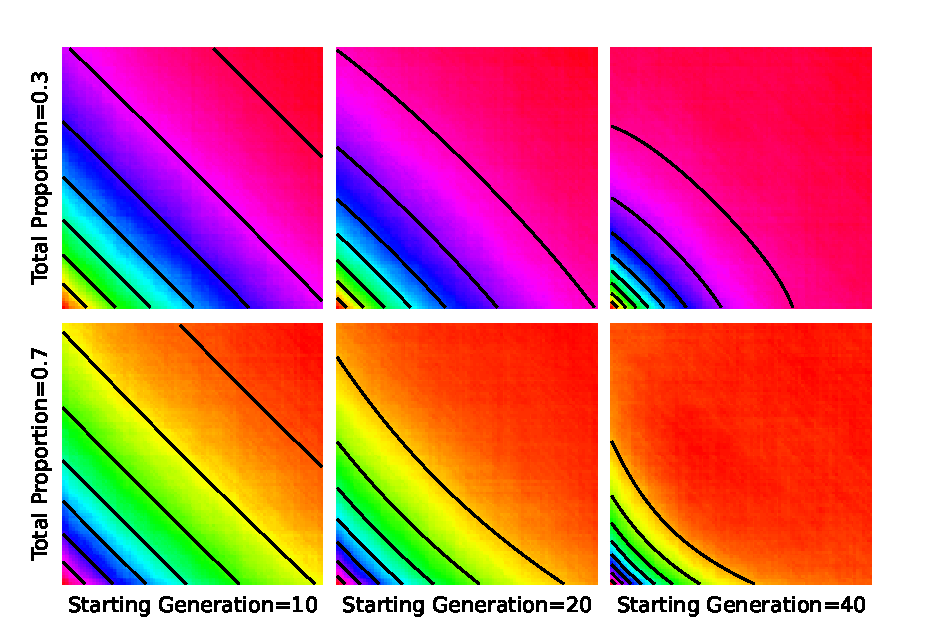
\includegraphics[scale=.8]{continuous.eps} \caption{ {\bf
Weighted LD surfaces produced by constant admixture.} The heat maps are from
simulations and the contours are from equation XX. In all six plots, admixture
stopped 5 generations before the present. Each square covers the range $0.5
\text{ cM }<d,d'<20\text{ cM}$. We varied the time of the beginning of the
admixture and the total admixture probability. The admixture probability for
each generation was constant, and chosen so that the total admixture proportion
was either $0.3$ or $0.7$. When the admixture is spread over 5 generations (the
leftmost column), the resulting weighted LD surface is similar to a one-pulse
weighted LD surface. For longer durations, the weighted LD surfaces are similar
to those produced by two pulses of admixture. } \label{continuous} \end{figure}

We first evaluate the accuracy of the equations developed in this paper by
comparing the analytical results to simulated data (Figures 1-3).  We find there
is a generally a close match between our equations and the simulated data under
both the two-pulse admixture scenarios (figures \ref{Ts} and \ref{ms}) and
constant-admixture scenarios (figure \ref{continuous}). The exception is when
the total admixture proportion $M_2+M_1(1-M_2)$ is close to 0.5. As the total
admixture proportion increases above 0.5, the contours for equation \ref{D3}
flip from being concave down to concave up. This transition can be seen by
comparing the upper left side of figure \ref{ms} to its lower right. At this
threshold, the contours of the estimated weighted LD depend on the actual
admixture fractions of the samples, which may differ from the expectation as a
result of genetic drift. This mismatch between theory and simulations is most
evident in figure \ref{ms}, for $m_1=0.1,m_2=0.4$ and $m_1=0.2,m_2=0.4$.

When there is continuous admixture scenario, the shape of the weighted LD
surface depends on both the duration and total amount of admixture. When the
duration is short, the weighted LD surfaces are indistinguishable from the
weighted LD surfaces produced by one pulse of migration. As the duration
increases, the contours of the weighted LD surface become more curved. The
contours are concave up when the total proportion is greater than $50\%$ and
concave down when it is less. When the total proportion is exactly $50\%$, the
amplitude of the weighted LD surface is much smaller than the sampling error.

For two pulse models, the effects of the second pulse of migration only become
evident when temporal spacing between the pulses is large enough ($T1 > T2$).
Otherwise, the resulting weighted LD surface cannot be distinguished from the
weighted LD surface produced by one pulse of admixture. As in the case of
continuous admixture the concavity of the surface contours is determined by the
total admixture proportion.

\begin{figure} 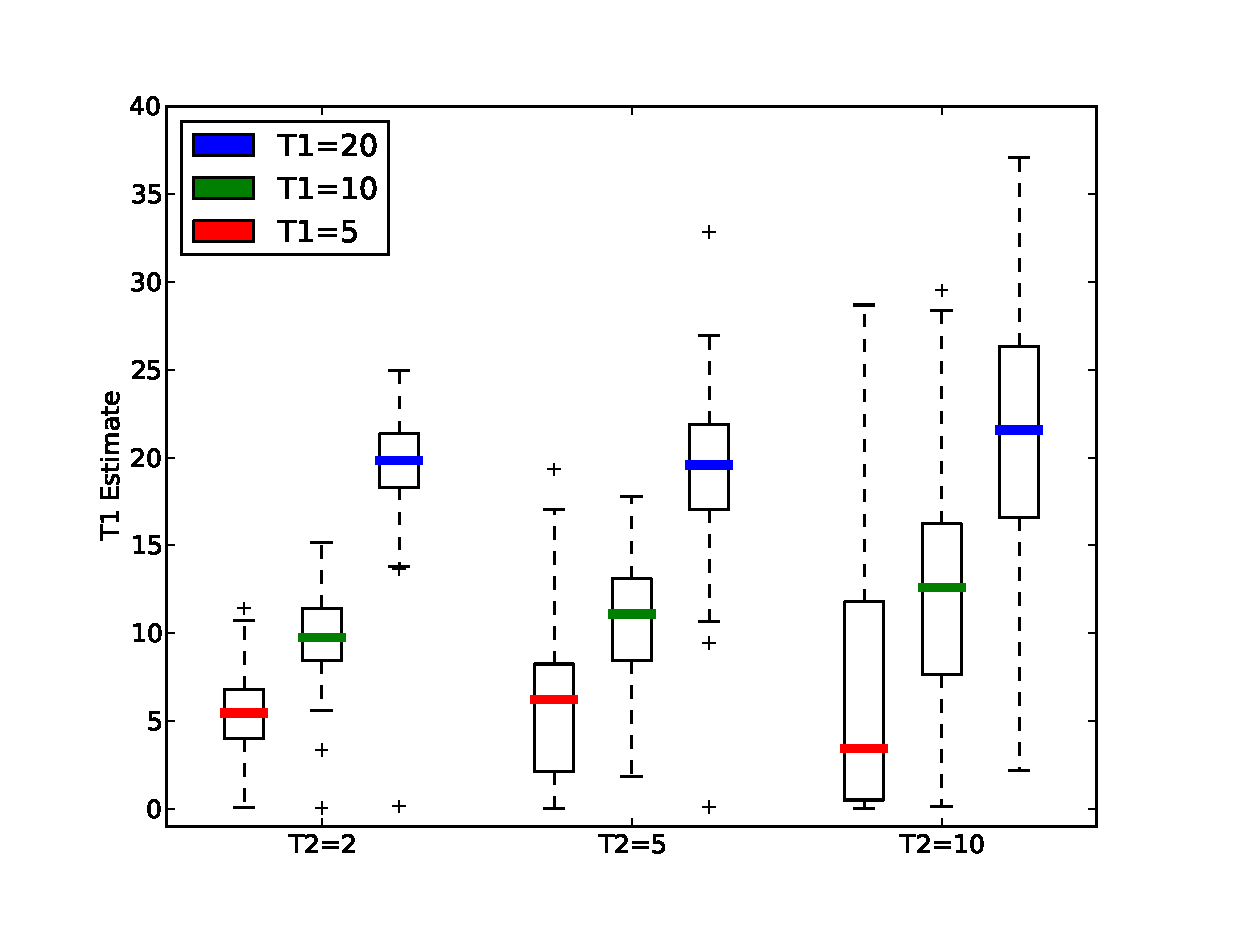
\includegraphics[scale=.6]{estimates.eps} \caption{ {\bf Accuracy
of estimates of $T_1$ as a function of other parameters.} Nine admixture
scenarios, $T_1\in \{5,10,20\}$ and $T_2\in\{2,5,10\}$, were simulated 100 times
each. The admixture probabilities were fixed at $M_1=0.3$ and $M_2=0.2$. The
colored bars give the medians of estimates for each of these nine cases, the
boxes delimit the interquartile range, and the whiskers extend out to 1.5 times
the interquartile range. As the time between the two pulses of admixture
increases, the error in the estimates decreases. Consistent with the simulations
shown in figure \ref{Ts}, there is limited power to estimate the time of the
more ancient admixture pulse when $T_2>T_1$. } \label{estimates} \end{figure}

[TODO Comment: we need  figures showing the similar one-dimensional LD for
comparison.  Maybe the first thing to discuss is to show how you can get
approximately the same 1D curve for different models which produce different 2D
surfaces]

We next evaluate the utility of the method for estimating admixture times.  The
qualitative similarities between one pulse and two pulse admixture scenarios
seen in the previous  simulations under some parameter settings, will naturally
affect  the estimates. As shown in figure \ref{estimates}, when the spacing
between the two pulses is small relative to their age, the median of the
estimates of the timing of the second pulse is close to the true value, but the
interquartile range is large. Moreover, the best fit often lies on a boundary of
the parameter space which is equivalent to a one pulse admixture model. When the
spacing between the pulses is larger, the estimates for the timing of the older
pulse becomes more precise. \subsection{1000 Genomes} \begin{figure}
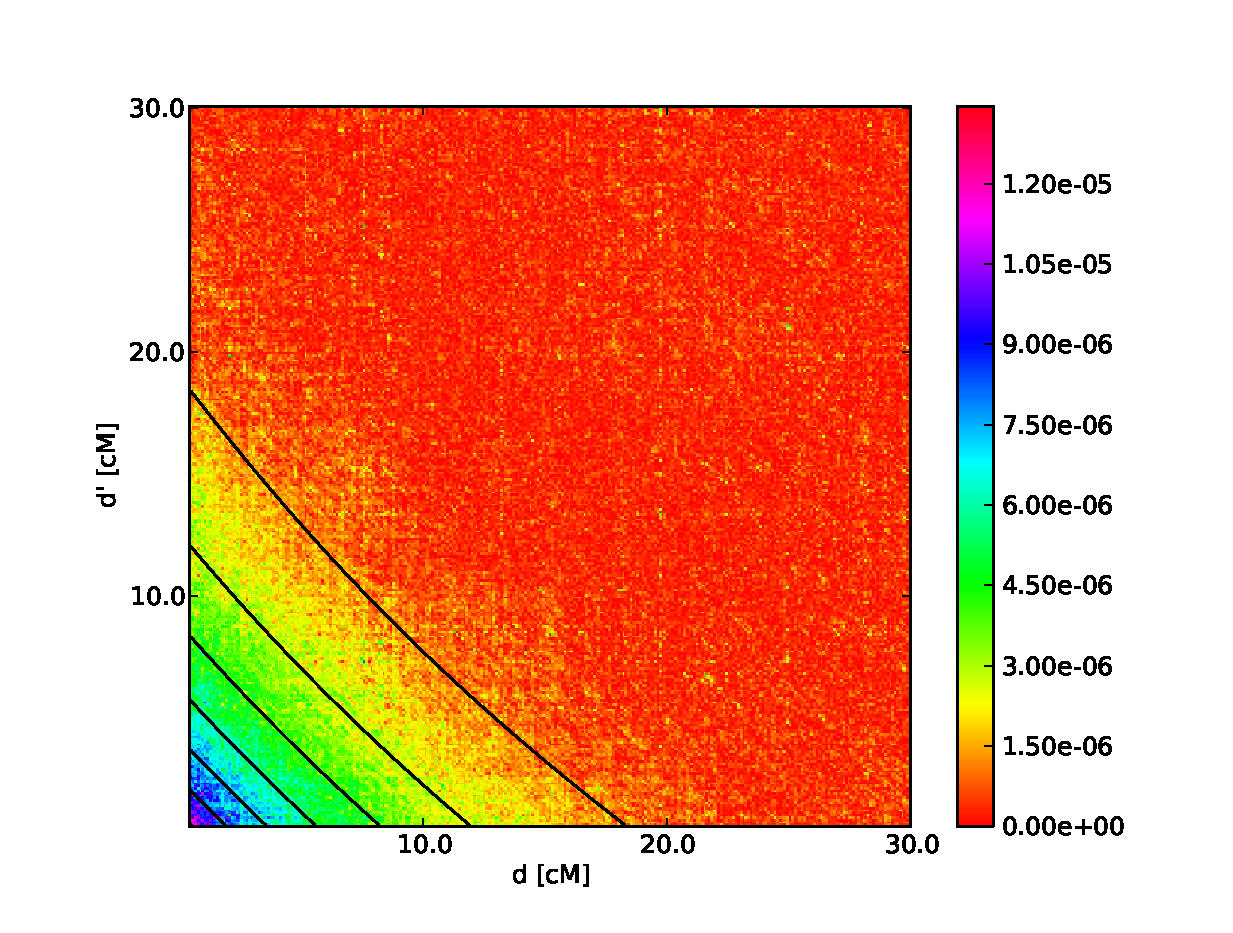
\includegraphics[scale=.6]{MXL.eps} \caption{ {\bf Weighted LD surface for
Mexican samples with Yoruba as reference.} The model with the best fit is two
pulses from the non-Yoruba source population at $T_1+T_2=12.3 \pm 3.3$ and
$T_2=9.9\pm 2.7$ generations ago. The jackknife confidence intervals for the
times of these two pulses overlap. } \label{ASH_MXL} \end{figure}

To illustrate the utility of the method we we computed weighted LD surfaces for
Mexican and Columbian samples from the 1000 Genomes consortium previously
analyzed for similar purposes by \cite{gravel2013reconstructing}. For the
Mexican samples, \cite{gravel2013reconstructing} found a small but consistent
amount of African ancestry, which appeared in the population 15 generations ago,
with continuing contributions from European and Native American populations
since that date, but no African migration. In fitting a two-pulse model to the
Mexican weighted LD surface (figure \ref{ASH_MXL}), we estimated that the two
pulses occurred $12.3\pm3.3$ and $9.9\pm2.7$ generations ago. These confidence
intervals overlap, and so we cannot reject a one-pulse admixture history. This
is not quite consistent with the constant migration model that
\cite{gravel2013reconstructing} found, but as we have seen from simulations, it
is hard to distinguish a constant migration model from a one-pulse model when
the duration of the migration is short.

\begin{figure} 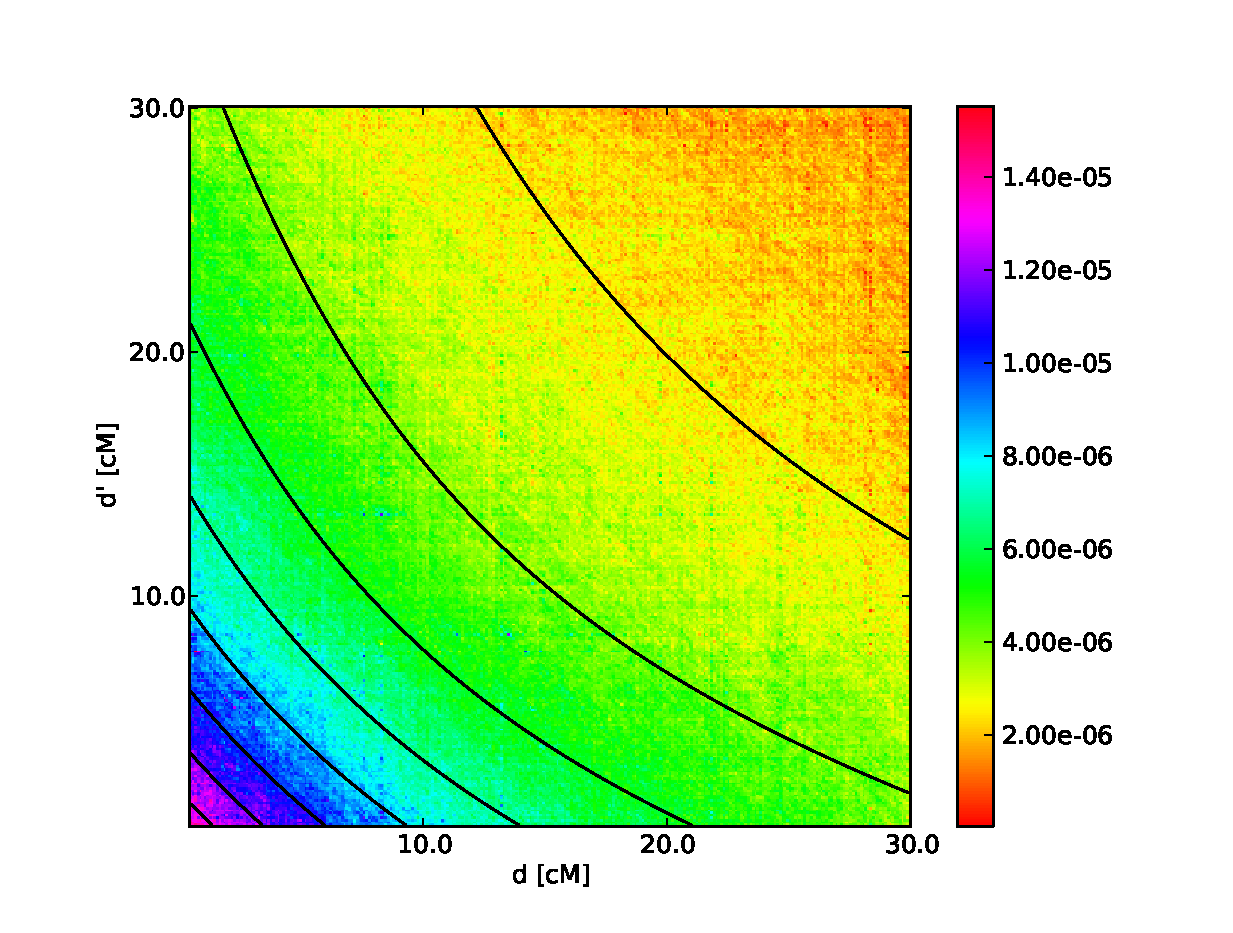
\includegraphics[scale=.6]{CLM.eps} \caption{ {\bf Weighted LD
surface for Colombian samples with Yoruba as reference} The two-pulse model that
fits best is two pulses of non-Yoruba admixture at $T_1+T_2=11.8\pm 1.2$ and
$T_2=2.64 \pm 0.08$ generations ago. The jackknife confidence intervals for the
times of these two pulses do not overlap. The amplitude of this weighted LD
surface is approximately ten times larger than that of the Mexican samples. This
a result of larger proportion of Yoruba ancestry in the Colombian samples. }
\label{ASH_CLM} \end{figure}

The weighted LD surface for the Columbia samples is shown in figure
\ref{ASH_CLM}. From this, we estimated two pulses of non-Yoruba migration at
$11.8\pm 1.2$ and $2.64\pm0.08$ generations before the present.
\cite{gravel2013reconstructing} also inferred two pulses of admixture,
corresponding to 3 and 9 generations ago. The weighted LD surface of the
Colombian samples has contours which are strongly concave up, in contrast to
those of the Mexican samples. \subsection{Comparison to Existing Methods}
Compared to existing weighted LD methods, our our method uses more information
in the data because it compares triples of SNPs instead of pairs. This gives our
method the ability to infer admixture histories more complex than a one-pulse
model. However, this comes at the price of greater estimation variances. ALDER
and ROLLOFF can make estimates from just tens of samples, while our method
requires hundreds of samples. Part of this difference can be attributed to the
fact that ALDER and ROLLOFF make inferences over a smaller class of models, but
the main reason arises from the fact that the existing two methods are
estimating second moments of the data, while we are estimating third moments.
The variance of these estimates are both inversely proportional to the sample
size, but the constants for estimating third moments are larger. As data becomes
more readily available, this disadvantage should disappear.

\bibliography{thesis}

\begin{figure}
	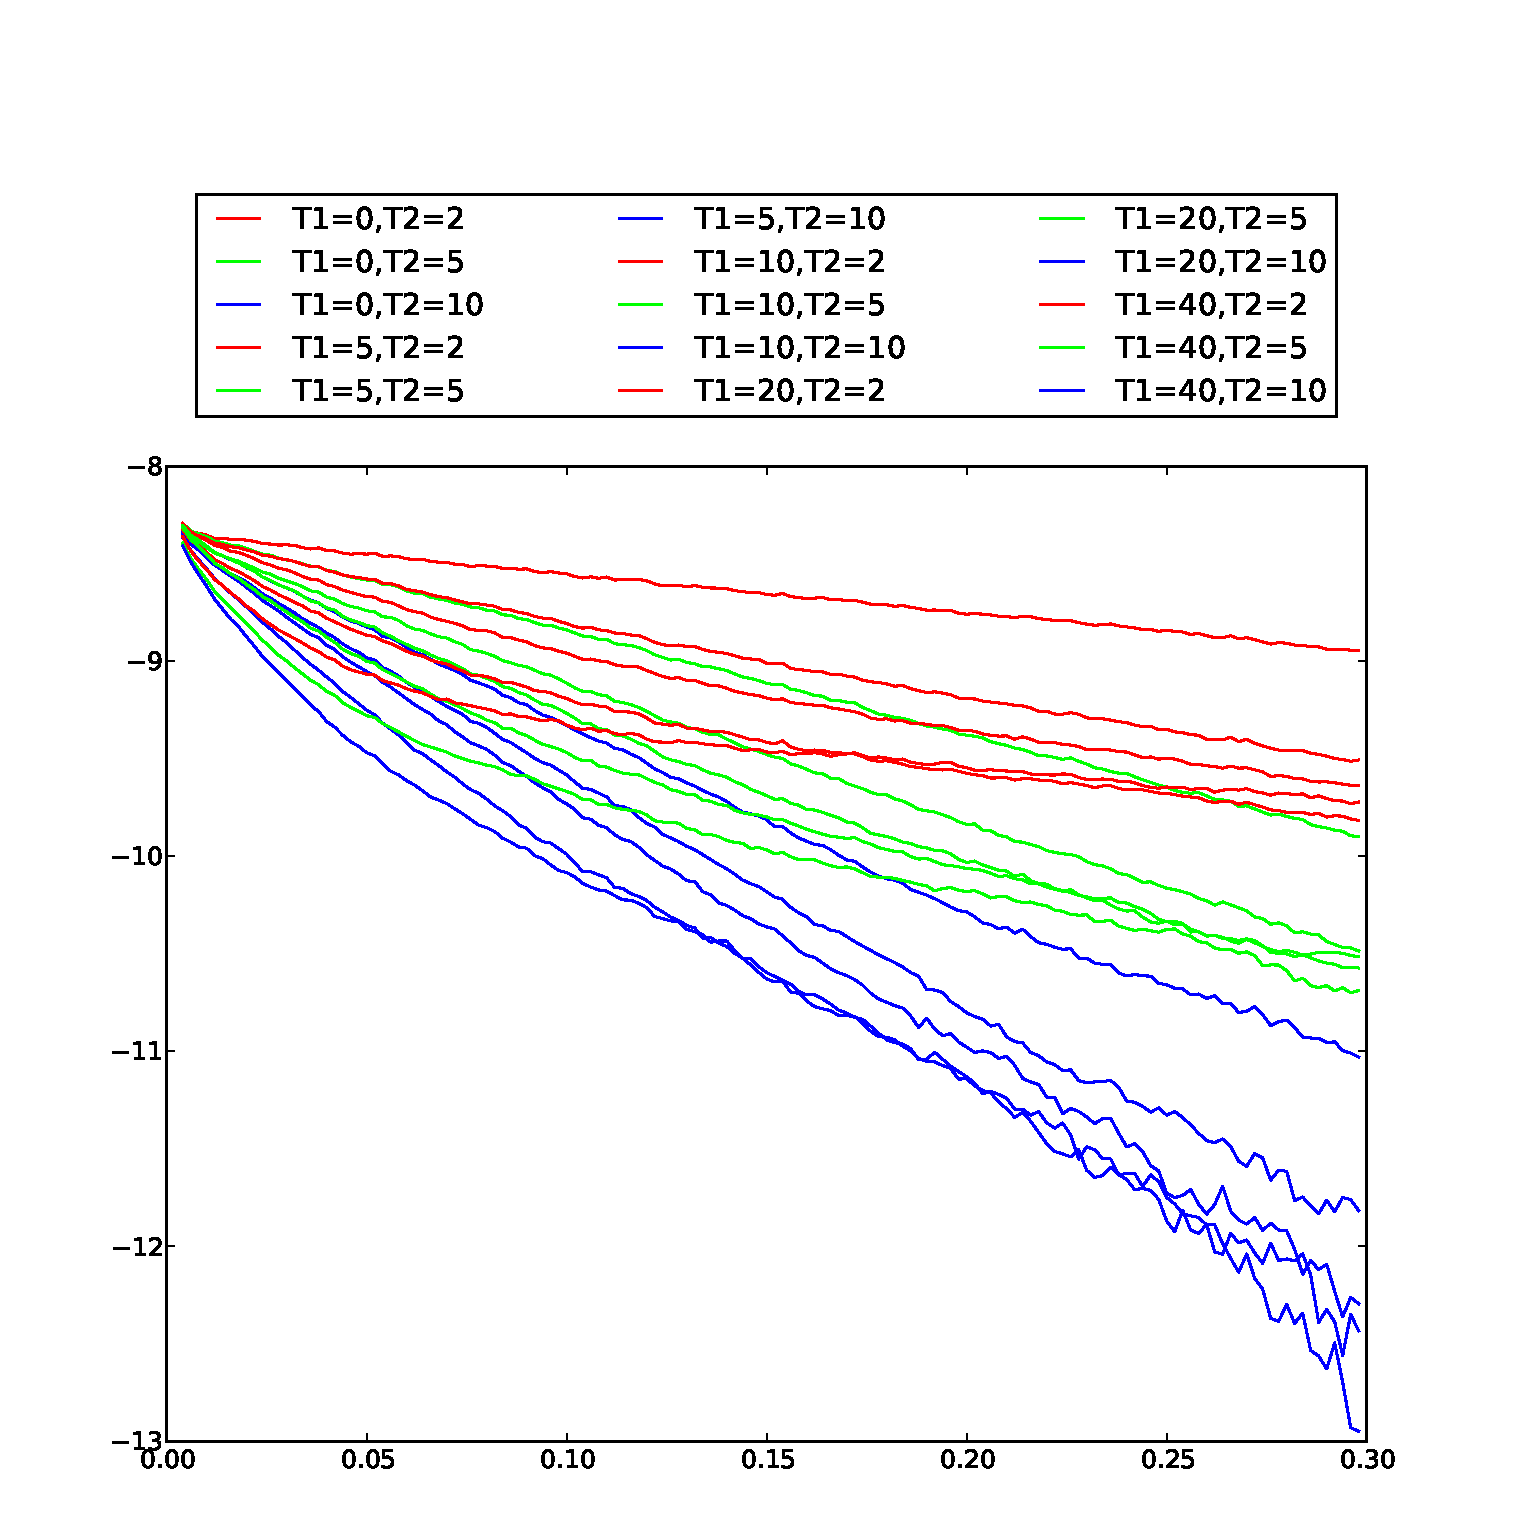
\includegraphics[scale=.6]{alder_Ts.eps}
	\caption{
		{\bf Extra figure}
		Corresponding Alder curves for two-pulse admixture with varying pulse times.
		Morgans on $x$-axis and $\log$ Alder scores on $y$-axis. Red lines are
		$T_2=2$, Green lines $T_2=5$, and blue lines are $T_2=10$.
	}
\end{figure}

\begin{figure}
	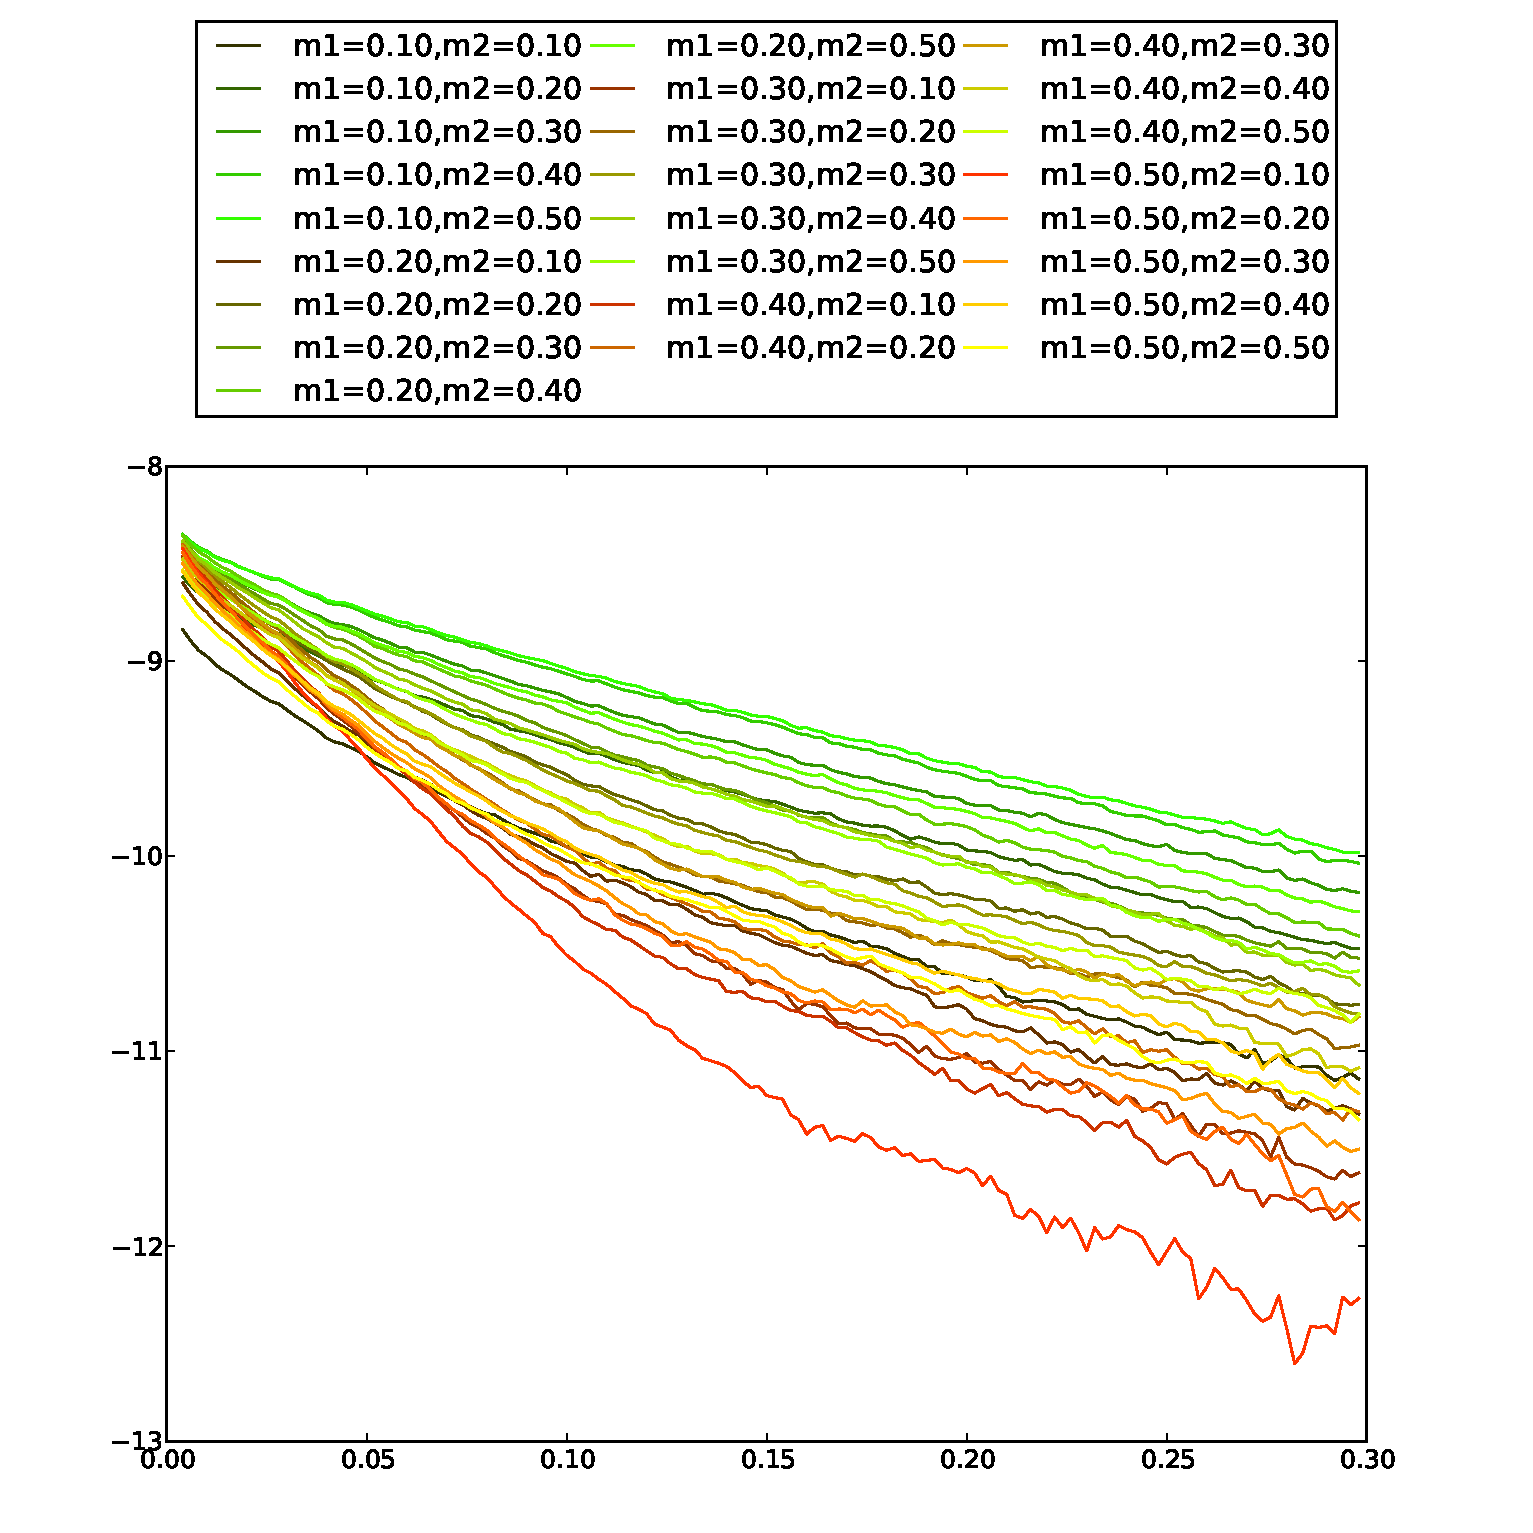
\includegraphics[scale=.6]{alder_ms.eps}
	\caption{
		{\bf Extra figure}
		Corresponding alder curves for two-pulse admixture with varying migration
		probabilities. Morgans on $x$-axis and $\log$ Alder scores on $y$-axis.
		Increasing red values are higher $M_1$'s and increasing green values are
		higher $M_2$'s  (TODO: choose better colors).
	}
\end{figure}

\end{document}
